\documentclass[11pt]{article}
\usepackage[margin=1in, top=1in]{geometry}
\usepackage[all]{nowidow}
\usepackage[hyperfigures=true, hidelinks, pdfhighlight=/N]{hyperref}
\usepackage[separate-uncertainty=true, group-digits=true]{siunitx}
\usepackage{graphicx,amsmath,physics,tabto,float,amssymb,pgfplots,verbatim,tcolorbox}
\usepackage{listings,xcolor,subfig,caption,import,wrapfig,enumitem}
\usepackage[version=4]{mhchem}
\usepackage[noabbrev]{cleveref}
\newcommand{\creflastconjunction}{, and\nobreakspace}
\newcommand{\mb}[1]{\mathbf{#1}}
\definecolor{stringcolor}{HTML}{C792EA}
\definecolor{codeblue}{HTML}{2162DB}
\definecolor{commentcolor}{HTML}{4A6E46}
\captionsetup{font=small, belowskip=0pt}
\lstdefinestyle{appendix}{
    basicstyle=\ttfamily\footnotesize,commentstyle=\color{commentcolor},keywordstyle=\color{codeblue},
    stringstyle=\color{stringcolor},showstringspaces=false,numbers=left,upquote=true,captionpos=t,
    abovecaptionskip=12pt,belowcaptionskip=12pt,language=Python,breaklines=true,frame=single}
\lstdefinestyle{inline}{
    basicstyle=\ttfamily\footnotesize,commentstyle=\color{commentcolor},keywordstyle=\color{codeblue},
    stringstyle=\color{stringcolor},showstringspaces=false,numbers=left,upquote=true,frame=tb,
    captionpos=b,language=Python}
\renewcommand{\lstlistingname}{Appendix}
\pgfplotsset{compat=1.17}

\begin{document}

\begin{center}
    \textbf{CP Exam}\hspace{1.5in}\textbf{KDSMIL001}\hspace{1.5in}\textbf{11-06-2022}
\end{center}
\rule{\textwidth}{1pt}

\begin{enumerate}
    \item \begin{enumerate}
        \item We generate \num[]{20000} random numbers according to the Gaussian distribution with form 
        \begin{equation}
            P_{\mathrm{Gaussian}}(N,\langle N \rangle)=\frac{1}{\sqrt{2\pi\langle N \rangle}}\exp\left(-\frac{(N-\langle N \rangle)^2}{2\langle N \rangle}\right)
            \label{eqn:gaussian}
        \end{equation}

        \begin{enumerate}
            \item The distribution of photon yields is shown in \cref{fig:q1a}, along with its expected heights. For use in following questions, the first number generated was $N=\num[]{9758.529}$, which rounds to $N=\num[]{9759}$.

            \begin{figure}[H]
                \begin{center}
                    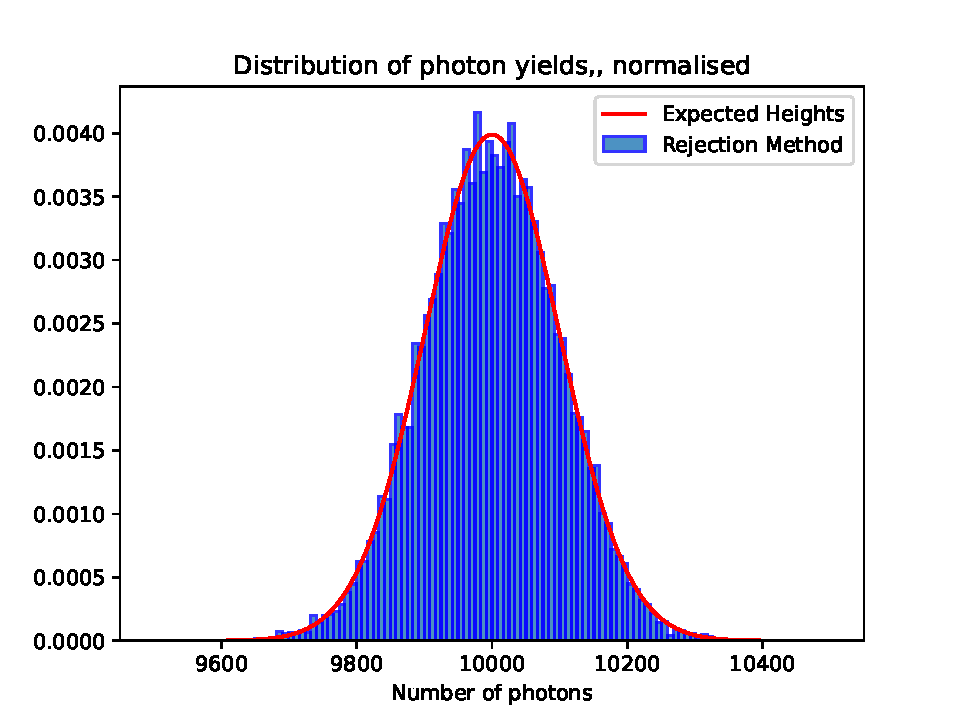
\includegraphics[width=.6\textwidth]{Plots/q1a.pdf}
                    \caption{Normalised distribution of photon yields. Expected heights are given by the Gaussian distribution in \cref{eqn:gaussian}.}
                    \label{fig:q1a}
                \end{center}
            \end{figure}
            
            \item The average yield was calculated to be \num[]{9999.4266}, which is round about what we expect.
            
            \item We found the variance to be \num{10020.466}. The assumed distribution has a variance of \num{10000}, so this is close, but it's hard to put an uncertainty on it so we can't say whether it's reasonable or not.
        \end{enumerate}

        \item We plot the distribution that photon momentum magnitudes obey, namely the Boltzmann distribution:
        \begin{equation}
            P(p)\propto p^2 e^{-p/T}
            \label{eqn:momentum magnitudes}
        \end{equation}

        \Cref{fig:q1b_unnormalised} shows the unnormalised distribution. Note that we plot it only on $p\in[0,30]$ as we can't plot it all the way to infinity, and it drops off appreciably by $p=30$. \\
        Integrating this distribution over $[0,\infty)$ we find a normalisation factor of 16, so we plot the normalised distribution in \cref{fig:q1b_normalised}, given by 
        \begin{equation}
            P(p)=\frac{p^2 e^{-p/T}}{16}.
            \label{eqn:boltzmann normalised}
        \end{equation}

        \begin{figure}[H]
            \begin{center}
                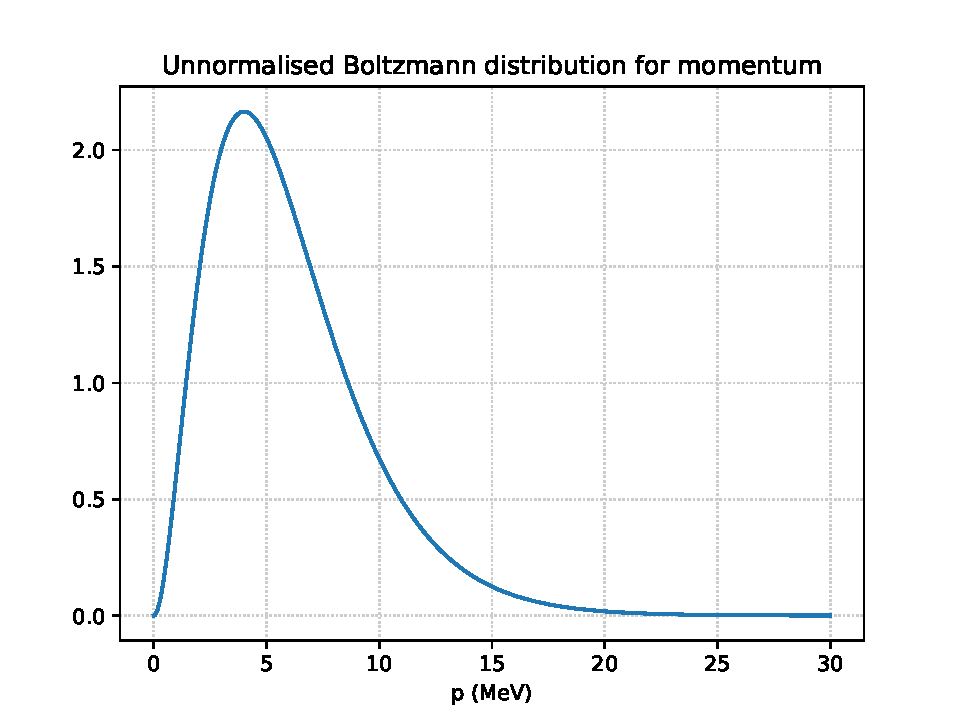
\includegraphics[width=.6\textwidth]{Plots/q1b_unnormalised.pdf}
                \caption{Unnormalised distribution of momentum magnitudes, following the Boltzmann distribution from \cref{eqn:momentum magnitudes} with $T=\SI{2}{\mega\electronvolt}$. }
                \label{fig:q1b_unnormalised}
            \end{center}
        \end{figure}

        
        \begin{figure}[H]
            \begin{center}
                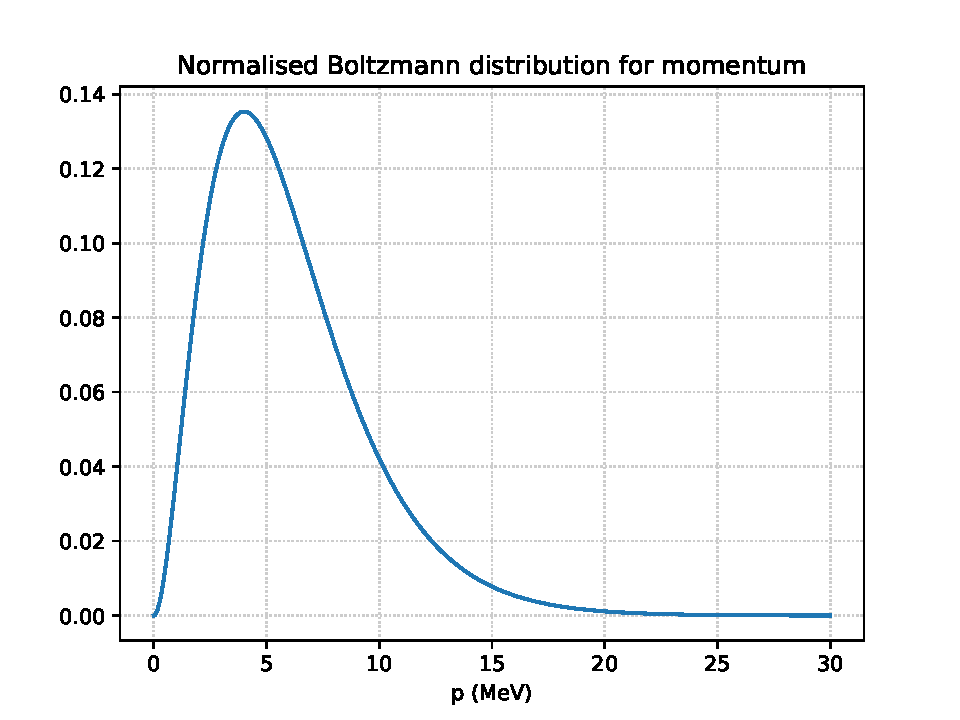
\includegraphics[width=.6\textwidth]{Plots/q1b_normalised.pdf}
                \caption{Normalised distribution of momentum magnitudes, once again following the distribution from \cref{eqn:momentum magnitudes} with $T=\SI{2}{\mega\electronvolt}$, now divided by 16.}
                \label{fig:q1b_normalised}
            \end{center}
        \end{figure}
        
        \item We now generate a set of random photon momentum magnitudes according to the distribution found above, specifically the normalised version. The number of photons to generate for is given by the first generated number in 1. a).
        
        \begin{enumerate}
            \item We plot the histogram in \cref{fig:q1c}
            \begin{figure}[h]
                \begin{center}
                    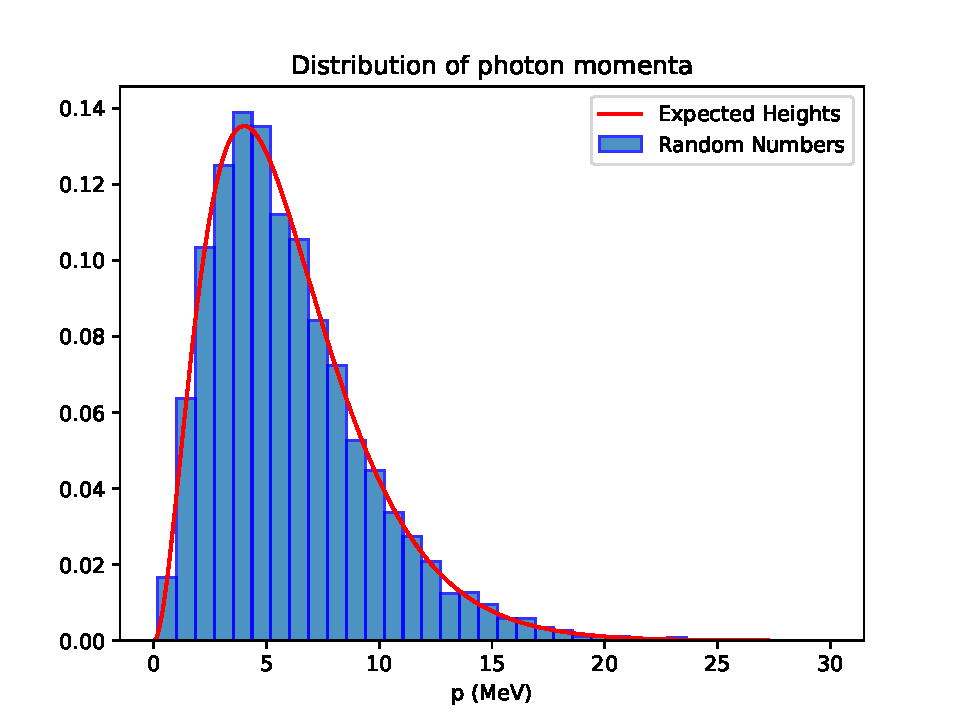
\includegraphics[width=.6\textwidth]{Plots/q1c.pdf}
                    \caption{Distribution of photon momentum magnitudes $p$, generated according to \cref{eqn:boltzmann normalised}, for \num{9759} photons. The expected heights are of course given by \cref{eqn:boltzmann normalised} as well.}
                    \label{fig:q1c}
                \end{center}
            \end{figure}

            \item The average $p$ was found to be \SI{5.9985}{\mega\electronvolt}.
            
        \end{enumerate}

        \item don't forget to derive these boys
        
        \item We aim to determine the expressions needed for the inverse method of generating random numbers. We begin with $\theta$.\\
        We can start with the general form of the inverse transform method
        \begin{equation}
            x_i=\int_{-\infty}^{y_i}P(y')dy'
            \label{eqn:general inverse method}
        \end{equation}
        where $x_i$ is a uniform number generated on $[0,1]$. We know that $\theta$ starts at 0, so we can write
        \begin{align*}
            x_i&=\int_0^{\theta_i}\frac 12 \sin\theta' d\theta'\\
            &=\frac 12 \left[-\cos\theta'\right]_0^{\theta_i}\\
            &=\frac 12 [-\cos\theta_i+1]\\
            \implies 2x_i-1&=-\cos\theta_i\\
            \implies \theta_i&=\arccos(1-2x_i).
        \end{align*}
        Now we can tackle $\phi$, once again starting \cref{eqn:general inverse method}. $\phi$ starts at $-\pi$, so we write
        \begin{align*}
            x_i&=\int_{-\pi}^{\phi_i}\frac{1}{2\pi}d\phi'\\
            &=\frac{1}{2\pi}[\phi']_{-\pi}^{\phi_i}\\
            &=\frac{1}{2\pi}[\phi_i+\pi]\\
            \implies2\pi x_i -\pi&=\phi_i\\
            \implies \phi_i &= 2\pi\left(x_i-\frac 12\right).
        \end{align*}

        \item We now use the inverse transform method to generate the distributions for $\theta$ and $\phi$ using the expressions found above. We will generate \num{9759} values as for the momentum magnitudes.
        \begin{enumerate}
            \item We plot the histograms
            
            \begin{figure}[h]
                \begin{center}
                    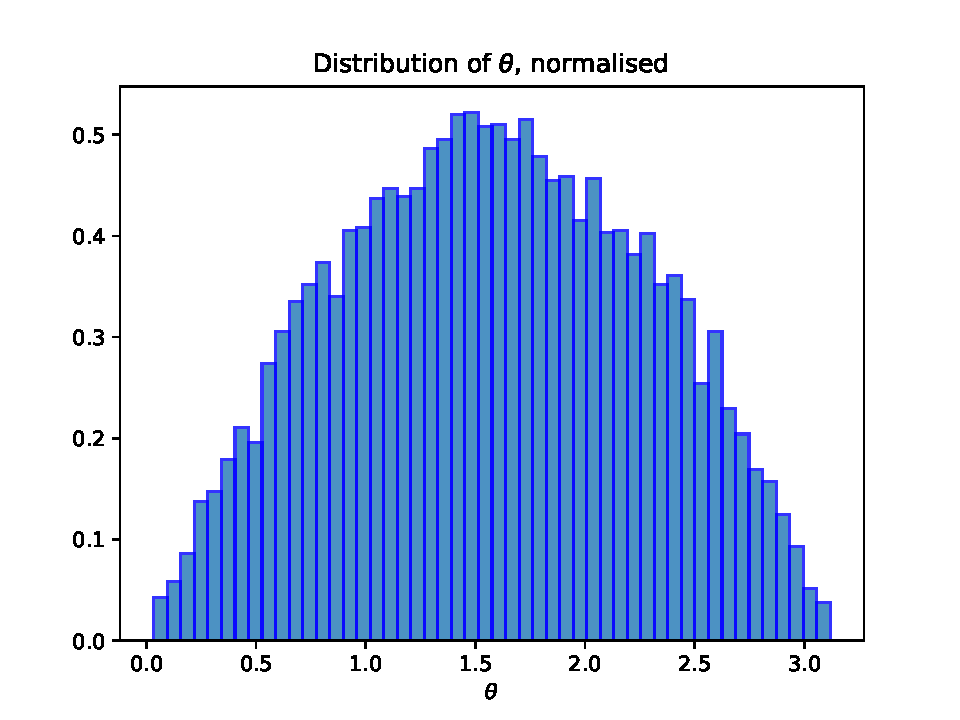
\includegraphics[width=.6\textwidth]{Plots/q1f_theta.pdf}
                    \caption{Distribution of \num{9759} random $\theta$ values generated with the inverse transform method.}
                    \label{fig:q1f theta}
                \end{center}
            \end{figure}

            \begin{figure}[h]
                \begin{center}
                    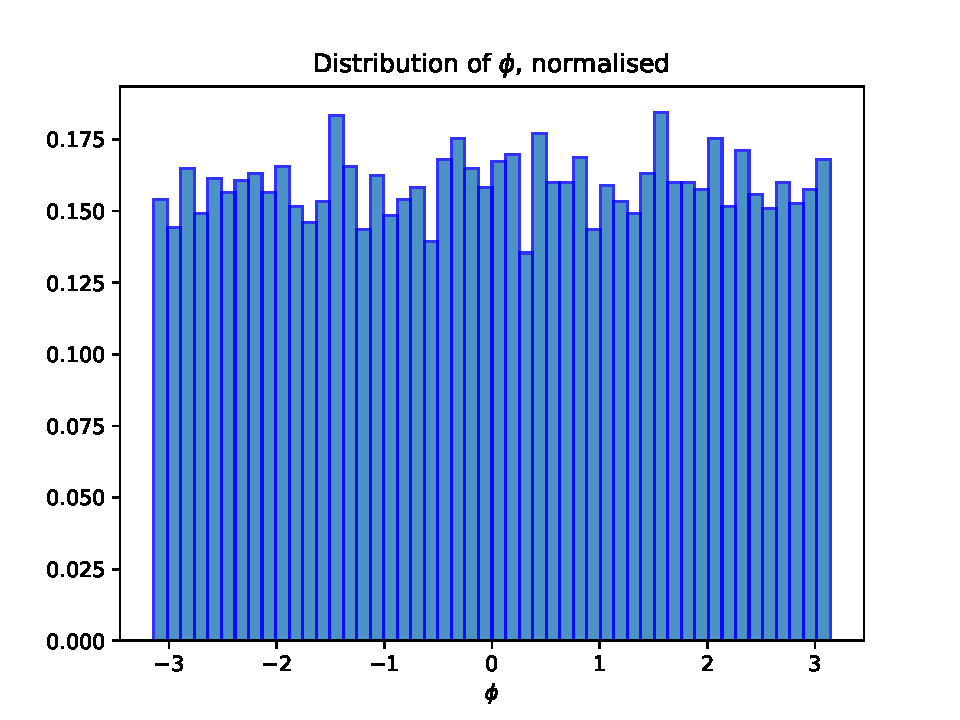
\includegraphics[width=.6\textwidth]{Plots/q1f_phi.pdf}
                    \caption{Distribution of \num{9759} random $\phi$ values generated with the inverse transform method.}
                    \label{fig:q1f phi}
                \end{center}
            \end{figure}
            
            \item We can find the average momentum in the $z$-direction for the first generated event. In spherical coordinates, the $z$ coordinate is given by 
            \begin{equation*}
                z=\cos\theta
            \end{equation*}
            so simply finding this value for each photon in the event and taking the mean we find $\langle p_z \rangle=\SI{-0.0007368}{\mega\electronvolt}$. 
            
        \end{enumerate}

        % -0.000736773019021856 z dir momentum
    \end{enumerate}
\end{enumerate}

\end{document}